\documentclass[11pt]{beamer}
% \usetheme{Boadilla}
  \usetheme{default}


% acronyms for text or math mode
\newcommand {\ccast} {\mbox{\small CCAST}}
\newcommand {\cris} {\mbox{\small CrIS}}

\newcommand {\airs} {\mbox{\small AIRS}}
\newcommand {\iasi} {\mbox{\small IASI}}
\newcommand {\idps} {\mbox{\small IDPS}}
\newcommand {\nasa} {\mbox{\small NASA}}
\newcommand {\noaa} {\mbox{\small NOAA}}
\newcommand {\nstar} {\mbox{\small STAR}}
\newcommand {\umbc} {\mbox{\small UMBC}}
\newcommand {\uw}   {\mbox{\small UW}}

\newcommand {\fft}  {\mbox{\small FFT}}
\newcommand {\ifft} {\mbox{\small IFFT}}
\newcommand {\fir}  {\mbox{\small FIR}}
\newcommand {\fov}  {\mbox{\small FOV}}
\newcommand {\for}  {\mbox{\small FOR}}
\newcommand {\ict}  {\mbox{\small ICT}}
\newcommand {\ils}  {\mbox{\small ILS}}
\newcommand {\igm}  {\mbox{\small IGM}}
\newcommand {\opd}  {\mbox{\small OPD}}
\newcommand {\rms}  {\mbox{\small RMS}}
\newcommand {\zpd}  {\mbox{\small ZPD}}
\newcommand {\ppm}  {\mbox{\small PPM}}
\newcommand {\srf}  {\mbox{\small SRF}}

\newcommand {\ES} {\mbox{\small ES}}
\newcommand {\SP} {\mbox{\small SP}}
\newcommand {\IT} {\mbox{\small IT}}
\newcommand {\SA} {\mbox{\small SA}}

\newcommand {\ET} {\mbox{\small ET}}
\newcommand {\FT} {\mbox{\small FT}}

% abbreviations, mainly for math mode
\newcommand {\real} {\mbox{real}}
\newcommand {\imag} {\mbox{imag}}
\newcommand {\atan} {\mbox{atan}}
\newcommand {\obs}  {\mbox{obs}}
\newcommand {\calc} {\mbox{calc}}
\newcommand {\sinc} {\mbox{sinc}}
\newcommand {\psinc} {\mbox{psinc}}
\newcommand {\std} {\mbox{std}}

% symbols, for math mode only
\newcommand {\wnum} {\mbox{cm$^{-1}$}}
\newcommand {\lmax} {L_{\mbox{\tiny max}}}
\newcommand {\vmax} {V_{\mbox{\tiny max}}}

\newcommand {\tauobs} {\tau_{\mbox{\tiny obs}}}
\newcommand {\taucal} {\tau_{\mbox{\tiny calc}}}
\newcommand {\Vdc}  {V_{\mbox{\tiny DC}}}

\newcommand {\rIT} {r_{\mbox{\tiny\textsc{ict}}}}
\newcommand {\rES} {r_{\mbox{\tiny\textsc{es}}}}
\newcommand {\robs} {r_{\mbox{\tiny obs}}}

\newcommand {\rITobs} {r_{\mbox{\tiny\textsc{ict}}}^{\mbox{\tiny obs}}}
\newcommand {\rITcal} {r_{\mbox{\tiny\textsc{ict}}}^{\mbox{\tiny cal}}}

\newcommand {\ITmean} {\langle\mbox{\small IT}\rangle}
\newcommand {\SPmean} {\langle\mbox{\small SP}\rangle}


\title{ccast NEdN estimate}
\author{H.~E.~Motteler and L.~L.~Strow}
\institute{
  UMBC Atmospheric Spectroscopy Lab \\
  Joint Center for Earth Systems Technology \\
}
\date{\today}
\begin{document}

%----------- slide --------------------------------------------------%
\begin{frame}[plain]
\titlepage
\end{frame}
%----------- slide --------------------------------------------------%
\begin{frame}
\frametitle{introduction}

\begin{itemize}
  \item the ccast NEdN estimate is derived from the calibration
    equation
  \item we describe the ccast estimate and compare it with the NOAA
    NEdN estimate
  \item although the methods differ in detail, results are similar
\end{itemize}

\end{frame}
%----------- slide --------------------------------------------------%
\begin{frame}
\frametitle{calibration equation}

The \ccast\ reference calibration equation is

\[\rES = F \cdot \rIT \cdot f \cdot \SA^{-1}\cdot f \cdot 
         \frac{\ES - \SPmean}{\ITmean - \SPmean} \]

\begin{itemize}
  \item $\rES$ is calibrated earth-scene radiance at the user grid
  \item $F$ is Fourier interpolation from sensor to user grid
  \item $f$ is a raised-cosine bandpass filter
  \item $\rIT$ is expected ICT radiance at the sensor grid
  \item $\SA^{-1}$ is the inverse of the ILS matrix
  \item $\ES$ is a single earth-scene count spectra
  \item $\ITmean$ is the mean of 9 ICT looks
  \item $\SPmean$ is the mean of 9 space looks
\end{itemize}

\end{frame}
%----------- slide --------------------------------------------------%
% \begin{frame}
% \frametitle{calibration equation}
% 
% \begin{itemize}
%   \item the $\IT$ and $\SP$ looks are averaged over several scans
%   \item a nonlinearity correction is applied to the ES, IT, and SP
%     count spectra
%   \item as part of that correction we divide the count spectra by
%     the numeric filter at the sensor grid, but this cancels out in
%     the ratio $(\ES - \SP) / (\IT - \SP)$
%   \item $F$ is a zero-filled double Fourier interpolation
%   \item $f \cdot \SA^{-1} \cdot f$ can be considered as a
%     physically-based smoothing of the rows and columns of $\SA^{-1}$
% \end{itemize}
% 
% \end{frame}
%----------- slide --------------------------------------------------%
\begin{frame}
\frametitle{NEdN estimate}

The NEdN estimate closely parallels the reference calibration
equation.  For each scan $i$ let

\[\rITobs(i) = \rITcal(i) \cdot f \cdot \SA^{-1}\cdot f \cdot 
               \frac{\IT(i) - \SPmean}{\ITmean - \SPmean} \]

\begin{itemize}
  \item $\rITobs(i)$ is calibrated ICT radiance
  \item $\rITcal(i)$ is expected ICT radiance
  \item $f$ is a raised-cosine bandpass filter
  \item $\SA^{-1}$ is the inverse of the ILS matrix
  \item $\ITmean$ is the mean of 60 ICT looks (one granule)
  \item $\SPmean$ is the mean of 60 space looks (one granule)
  \item $\rITobs(i)$ is calculated at the sensor grid for each 
    FOV and both sweep directions
\end{itemize}

\end{frame}
%----------- slide --------------------------------------------------%
\begin{frame}
\frametitle{NEdN estimate}

\begin{itemize}
  \item for each FOV and sweep direction let $N_1 = \std(\rITobs)$
    be the standard deviation of $\rITobs$ for all scans from one
    granule

  \item this is a conventional noise estimate, but the estimate
    itself is too noisy

  \item we apply a principle component filter to $N_1$, as follows

  \item let $U$ be an $n$ by $k$ matrix consisting of the first $k$
    left singular vectors of a significant sample of $N_1$
    estimates.  We used 540 values from 540 consecutive granules

  \item $k$ is chosen by examining singular values and vectors.  
    For initial tests we chose $k = 6$ for the LW band, $5$ for 
    the MW, and $4$ for the SW

  \item then $N_2 = U \cdot U^T \cdot N_1$ gives the desired NEdN
    estimate
\end{itemize}

\end{frame}
%----------- slide --------------------------------------------------%
\begin{frame}
\frametitle{NOAA NEdN estimate}

\begin{itemize}
  \item The NOAA NEdN estimate is generally similar
  \item $N_1$ is calculated as above from a 30-scan moving window
    rather than once per 60-scan granule.  
  \item The $N_1$ values (one per scan) are then averaged with a
    17-element moving window to give one smoothed estimate per scan.
  \item despite differences in the calculation methods, the ccast
    and NOAA NEdN estimates are in reasonable agreement
  \item the following figures show ccast and NOAA estimates for the
    same granule, for all 9 FOVs and three bands

\end{itemize}

\end{frame}
%----------- slide --------------------------------------------------%
\begin{frame}
\frametitle{NOAA LW NEdN detail}

\begin{center}
  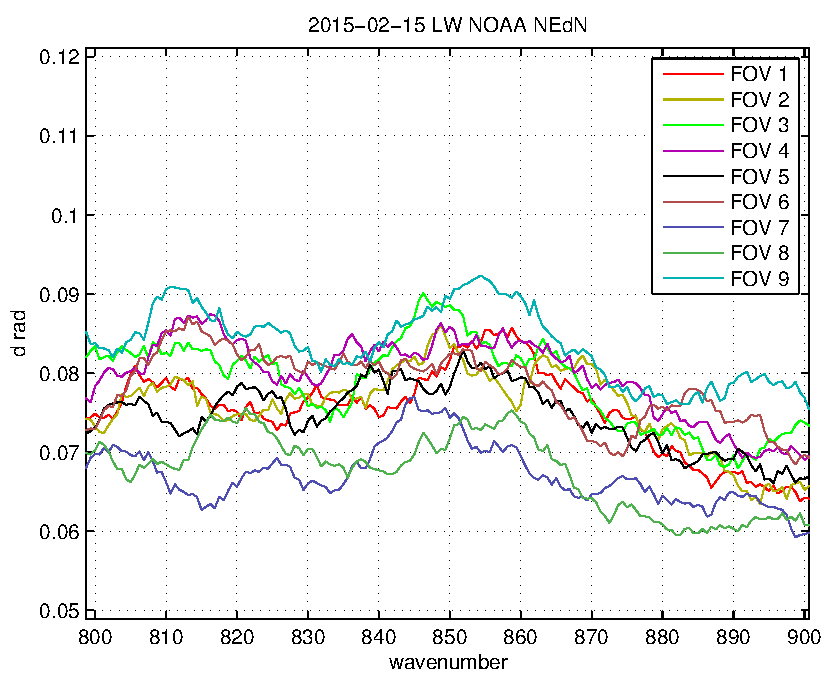
\includegraphics[scale=0.54]{figures/nedn_noaa_LW.pdf}
\end{center}

\centerline{zoom of a representative LW NOAA NEdN estimate}

\end{frame}
%----------- slide --------------------------------------------------%
\begin{frame}
\frametitle{ccast LW NEdN detail}

\begin{center}
  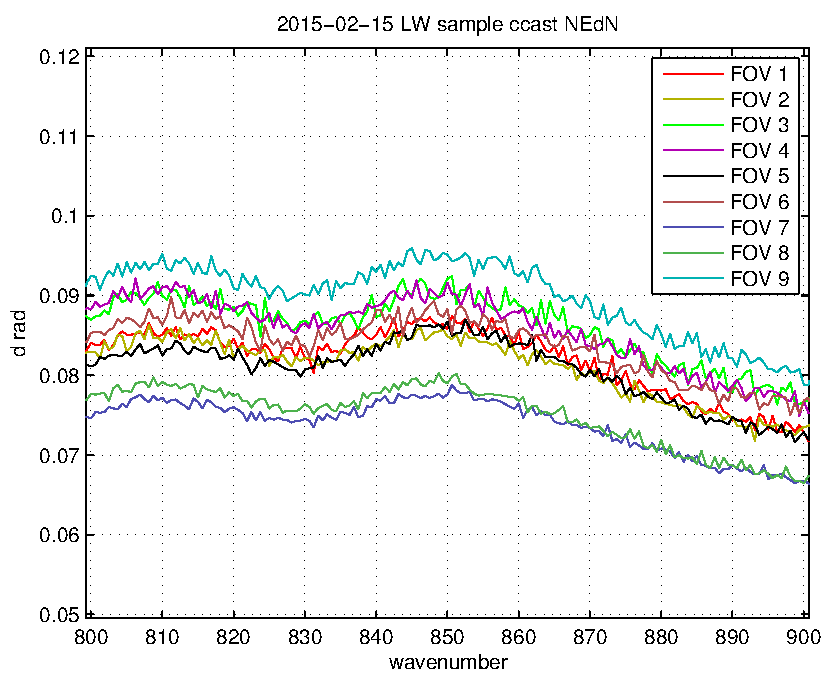
\includegraphics[scale=0.54]{figures/nedn_ccast_LW.pdf}
\end{center}

\centerline{the corresponding ccast estimate is slightly higher}

\end{frame}
%----------- slide --------------------------------------------------%
\begin{frame}
\frametitle{NOAA MW NEdN sample}

\begin{center}
  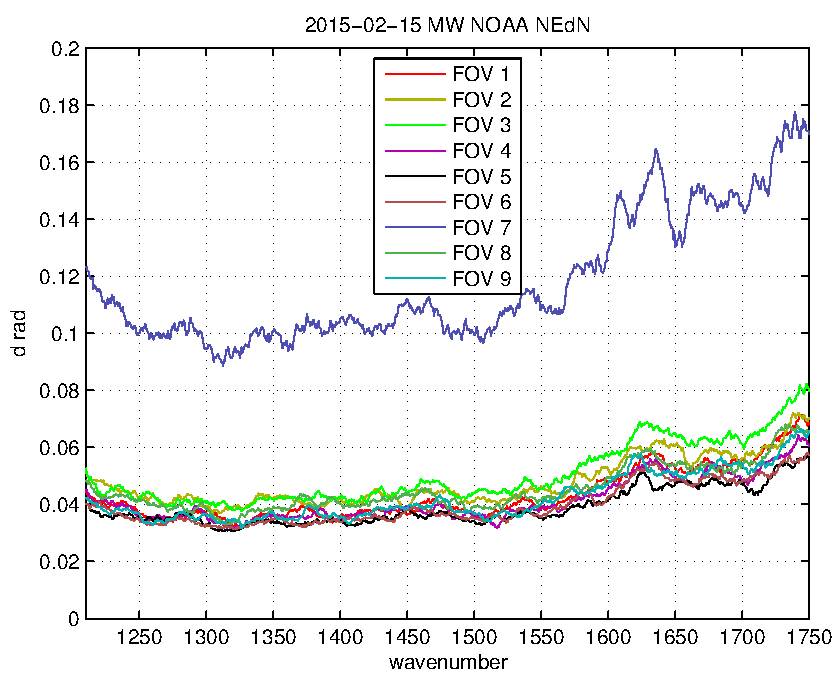
\includegraphics[scale=0.54]{figures/nedn_noaa_MW.pdf}
\end{center}

\centerline{MW FOV 7 is significantly less linear}

\end{frame}
%----------- slide --------------------------------------------------%
\begin{frame}
\frametitle{ccast MW NEdN sample}

\begin{center}
  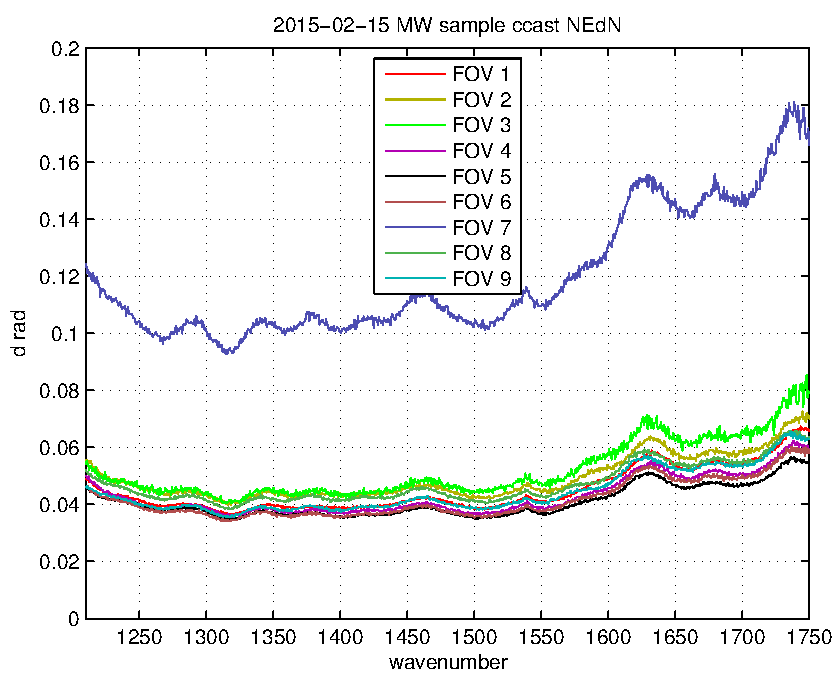
\includegraphics[scale=0.54]{figures/nedn_ccast_MW.pdf}
\end{center}

\centerline{the corresponding ccast estimate is quite close}

\end{frame}
%----------- slide --------------------------------------------------%
\begin{frame}
\frametitle{NOAA SW NEdN sample}

\begin{center}
  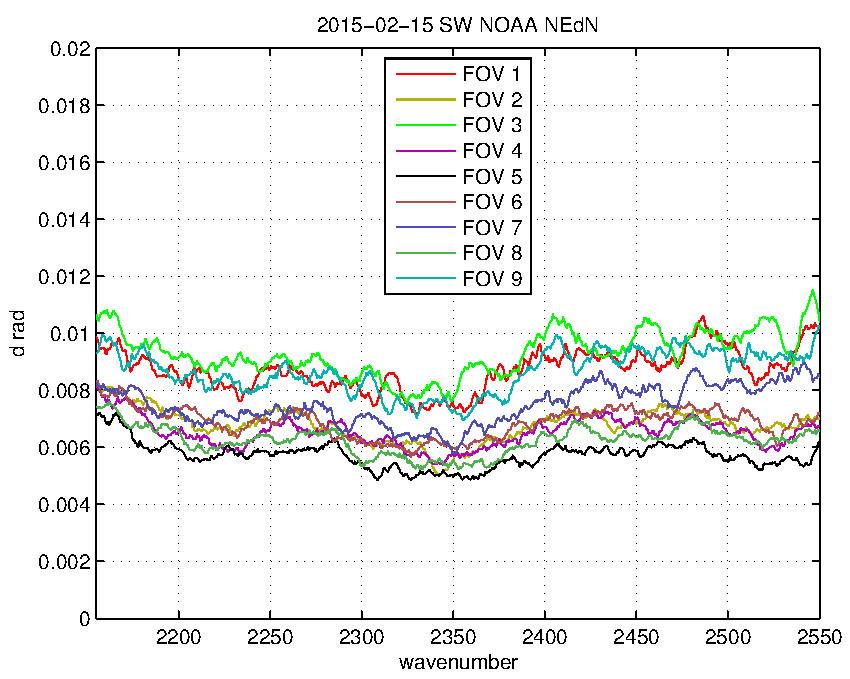
\includegraphics[scale=0.54]{figures/nedn_noaa_SW.pdf}
\end{center}

\end{frame}
%----------- slide --------------------------------------------------%
\begin{frame}
\frametitle{ccast SW NEdN sample}

\begin{center}
  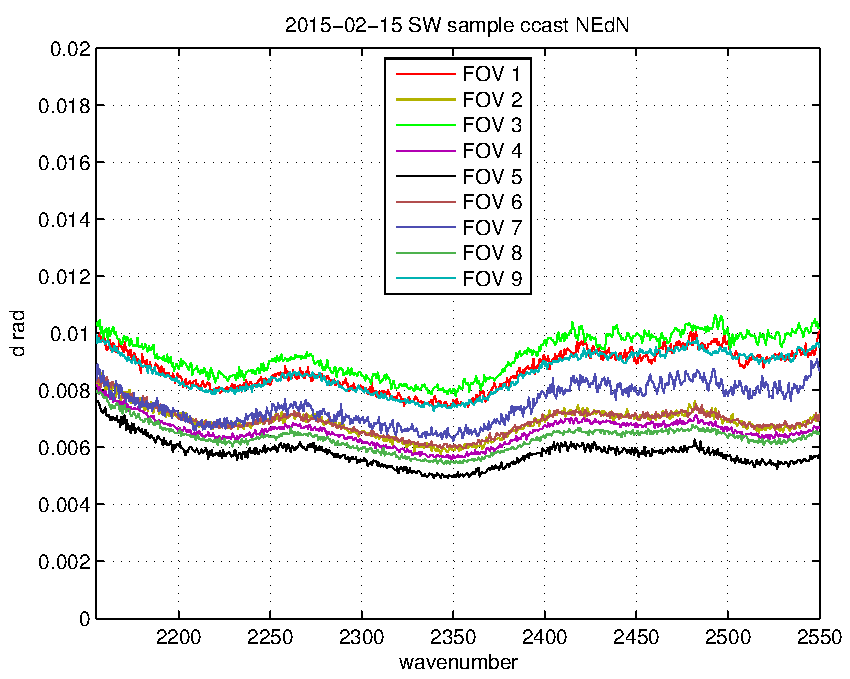
\includegraphics[scale=0.54]{figures/nedn_ccast_SW.pdf}
\end{center}

\end{frame}
%----------- slide --------------------------------------------------%
\begin{frame}
\frametitle{conclusions}

\begin{itemize}

  \item the ccast and NOAA NEdN estimates are generally in good
    agreement 

  \item the NOAA estimate has more low-frequency noise, and the
    ccast estimate more high-frequency noise

  \item the NOAA and ccast results shown here are from the high
    resolution prototypes.  The regular resolution estimates are
    also similar
\end{itemize}

\end{frame}
%----------- slide --------------------------------------------------%
\end{document}

